\documentclass{standalone}
\usepackage{tikz}
\begin{document}

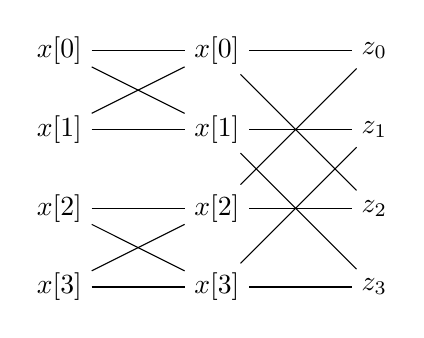
\begin{tikzpicture}
    % Nodes
    \node (a0) at (0,2) {$x[0]$};
    \node (a1) at (0,1) {$x[1]$};
    \node (a2) at (0,0) {$x[2]$};
    \node (a3) at (0,-1) {$x[3]$};

    \node (b1) at (2, 2) {$x[0]$};
    \node (b2) at (2, 1) {$x[1]$};
    \node (b3) at (2, 0) {$x[2]$};
    \node (b4) at (2,-1) {$x[3]$};

    \node (c1) at (4, 2) {$z_0$};
    \node (c2) at (4, 1) {$z_1$};
    \node (c3) at (4, 0) {$z_2$};
    \node (c4) at (4, -1) {$z_3$};

    % Lines
    \draw[-] (a0) -- (b1);
    \draw[-] (a1) -- (b2);
    \draw[-] (a2) -- (b3);
    \draw[-] (a3) -- (b4);

    \draw[-] (b1) -- (c1);
    \draw[-] (b2) -- (c2);
    \draw[-] (b3) -- (c3);
    \draw[-] (b4) -- (c4);

    \draw[-] (a0) -- (b2);
    \draw[-] (a1) -- (b1);
    \draw[-] (a2) -- (b4);
    \draw[-] (a3) -- (b3);

    \draw[-] (b1) -- (c3);
    \draw[-] (b2) -- (c4);
    \draw[-] (b3) -- (c1);
    \draw[-] (b4) -- (c2);
\end{tikzpicture}

\end{document}
